\documentclass{article}
\usepackage[utf8]{inputenc}
\usepackage[margin=1in]{geometry}
\usepackage[titletoc,title]{appendix}
\usepackage{amsmath,amsfonts,amssymb,mathtools}
\usepackage{graphicx,float}
\usepackage[ruled,vlined]{algorithm2e}
\usepackage{algorithmic}
\usepackage{biblatex}
\usepackage{tikz}
\usepackage{matlab-prettifier}
\usepackage{listings}
\usepackage{xcolor}
\usepackage{hyperref}
\usepackage{caption}
\usepackage{subfig}
\usepackage[parfill]{parskip}
\addbibresource{references.bib}

\newcommand{\hmwkTitle}{Final Project}
\newcommand{\hmwkDueDate}{March 19, 2020}
\newcommand{\hmwkClass}{Computational Methods for Data Analysis}
\newcommand{\hmwkClassNum}{AMATH 582}
\newcommand{\hmwkClassInstructor}{Professor J. Nathan Kutz}
\newcommand{\hmwkAuthorName}{\textbf{Chandan Sharma Subedi}}
\newcommand{\hmwkClassSection}{Section A}

%
% Title Page
%

\title{
    \vspace{2in}
    \textmd{\textbf{\hmwkClass}}\\
    \vspace{0.3in}\textmd{\textbf{\hmwkTitle}}\\
    \normalsize\vspace{0.1in}\small{Due\ on\ \hmwkDueDate\ at 5:00pm}\\
    \vspace{0.1in}\large{\textit{\hmwkClassInstructor}} \\
    \vspace{0.1in}\large{{\hmwkClassSection}} \\
    \vspace{2.5in}
}

\author{\hmwkAuthorName}
\date{}

\begin{document}

\maketitle
\pagebreak

% Abstract
\begin{abstract}
In this paper, Singular Value Decomposition is applied to stabilize a video, captured with a hand-held camera, while walking. Optical flow is estimated between two consecutive frames to construct the matrix. Left singular matrix is used to identify the mode associated with pixels moving up and down due to the act of walking. The video is then reconstructed using first few principal components. Lucas-Kanade and Horn-Schunck methods are experimented using MATLAB built-in functions for better optical flow estimates.
\end{abstract}

% Introduction and Overview
\section{Introduction and Overview}
Everyday Terabytes of videos are captured all over the world across many devices. This has attracted the development of many video stabilization softwares. The iPhone has it's own video stabilization software that runs in real-time as you take the video. In this paper, an attempt has been made to investigate the application of SVD to stabilize a particular type of instability, distortions on the video due to walking motion. When a person walking on the road captures a video through a hand-held camera, you see images shifting up and down on the video. Is there a way we can identify that motion and remove it from the video?

A concept of Optical Flow is introduced that identifies how each pixels are moving between two consecutive frames. Using this velocity data, two matrices are constructed, each corresponding to $x$-direction and $y$-direction. Singular Value Decomposition is used to extract information from these matrices. Section \ref{Theory} lays down theoretical foundation behind Optical Flow and SVD, while section \ref{Algorithm} describes algorithms used for the analysis. Section \ref{Result} put forwards the result of analysis.

%  Theoretical Background
\section{Theoretical Background}\label{Theory}
Optical flow is the motion of pixels between consecutive image frames, caused by the relative movement between the scene and the camera. It measures the velocity of each pixel in the image. Let $I(x,y,t)$ be the intensity of an image as a function of space $(x,y)$ and time $(t)$. If image is dispaced by $(\delta x,\delta y)$ over time $t$, the new image obtained is $I(x+\delta x, y+\delta y, t+\delta t)$. It is assumed that the intensities of the object do not change between consecutive frames. Thus,
\[
I(x,y) = I(x+dx, y+dy, t+dt)
\]
The Taylor series expansion of RHS about the point $(x,y,t)$ gives us,
\begin{align*}
I(x,y,t) &= I(x,y,t) + \frac{\partial I}{\partial x} \delta x + \frac{\partial  I}{\partial y} \delta y + \frac{\partial  I}{\partial t} \delta t + ... \\
&\implies \frac{\partial I}{\partial x} \delta x + \frac{\partial  I}{\partial y} \delta y + \frac{\partial  I}{\partial t} \delta t = 0
\end{align*}
Dividing by $dt$, we get the optical flow equation:
\[
 \frac{\partial I}{\partial x}u +  \frac{\partial I}{\partial y}v +  \frac{\partial I}{\partial t} = 0
\]
This equation cannot be solved directly since we have two unknowns $(u,v)$, that specify the velocity of a pixel, but one equation. 
Lucas-Kanade and Horn-Schunck method are two techniques to compute sparse optical flow. Under Lucas-Kande method a $3x3$ patch of pixels are considered, instead of one, and it is assumed that all $9$ pixels in the patch have the same velocities. This gives us an over-defined system of $9$ linear equations that can be solved using least-square method.
\begin{align*}
Ax &= b \\
\begin{bmatrix}
I_x(q_1) & I_y(q_1) \\
I_x(q_2) & I_y(q_2) \\
\vdots & \vdots   \\
I_x(q_9) & I_y(q_9)
\end{bmatrix}
\begin{bmatrix}
V_x \\
V_y\\
\end{bmatrix}
&=
\begin{bmatrix}
-I_t(q_1) \\
-I_t(q_2) \\
\vdots \\
-I_t(q_9)
\end{bmatrix}
\end{align*}
Singular Value Decomposition is a matrix decomposition of the form
\begin{align*}
\begin{bmatrix}
&&\\
&&\\
&\textbf{A}& \\
&&\\
&&\\
\end{bmatrix}
\begin{bmatrix}
&&\\
&&\\
&\mathbf{v_1}& \mathbf{v_2}& \hdots & \mathbf{v_n}&\\
&&\\
&&\\
\end{bmatrix}
&=
\begin{bmatrix}
&&\\
&&\\
&\mathbf{u_1}& \mathbf{u_2}& \hdots & \mathbf{u_n}&\\
&&\\
&&\\
\end{bmatrix}
\begin{bmatrix} 
\mathbf{\sigma_1}&&\\
&\mathbf{\sigma_2}&\\
&& \ddots \\
&&&& \\
&&&&\mathbf{\sigma_n}\\
\end{bmatrix} \\
\mathbf{AV} &= \mathbf{U\Sigma} \\
\mathbf{A} &= \mathbf{U\Sigma V^{*}}
\end{align*}
The matrix $\mathbf{\Sigma}$ is an $m$ x $n$ diagonal matrix with positive entries provided the matrix \textbf{A} is of full rank. It stores the singular values, representing the stretching space, ordered from largest to smallest so that $\sigma_1 \ge \sigma_2 \ge ... \ge \sigma_n$. The matrix \textbf{U} is a $m$ x $n$ unitary matrix with orthonormal columns (left-singular vectors). The matrix \textbf{V} is an $n$ x $n$ unitary matrix with orthonormal columns (right-singular vectors). Both of these vectors represent rotation. Furthermore, $\mathbf{v_1}$ is the vector that, when multiplied with the matrix A, strectches by a factor of $\mathbf{\sigma_1}$ and rotates so that it points along $\mathbf{u_1}$. Therefore columns of matrix \textbf{V} are the principal components of the matrix \textbf{A}. \\

% Algorithm Implementation and Development
\section{Algorithm Implementation and Development}\label{Algorithm}
The analysis primarily constituted five steps: \\

\textbf{Data Collection and Formatting} \\
A video was downloaded from the Youtube, where a person is walking around the city with a camera held on his hand. The video captured was relatively stable in all directions except in the vertical direction where frames were moving up and down because of walking motion. The video was loaded and each image was grayscaled and downscaled by a factor of $1/4$ to obtain $270$ x $480$ frame. \\

\textbf{Optical Flow Estimation} \\
MATLAB in-built command \emph{estimateFlow} is used to estimate the flow matrix. Lucas-Kanade and Horn-Schunck methods are implemented using in-built objects \emph{opticalFlowLK} and \emph{opticalFlowHS} as command parameters. It returns a dense optical flow estimates $(V_x, V_y)$ at each pixel. \\

\textbf{Matrices Construction and SVD}\\
Two matrices corresponding to the flow estimates alongs $x$-direction and $y$-direction are transformed into column vectors. Two matrices $F_X$ and $F_Y$ are constructed such that their columns represent flow estimate matrix of each frames along $x$ and $y$ directions respectively. Each matrices is normalized to zero mean. Economic SVD is implemented on these matrices using MATLAB in-built command \emph{svd}. \\

\textbf{Video Reconstruction} \\
Each image frame is warped using a low-rank approximation of the optical flow estimates. While the initial intent was to identify singular modes associated with distortions in the image due to walking, it became clear after implementation that isolating those modes is not easy, especially when modes are two dimensional $(u,v)$. Therefore reconstruction was done simply by taking low-rank approximations.


% Computational Results
\section{Computational Results}\label{Result}
A long video is downloaded such that the analysis can be performed on different sections of the video. The video can be found on \href{https://www.youtube.com/watch?v=hNuVhnMWYhA}{Youtube} and is $\approx 35$ mins long. After video is loaded and image is formatted, optical flow is estimated. Figure \ref{fig:flow} (a) and (b) show those estimates for Lucas-Kanade and Horn-Schunck method. Horn-Schunck method gives better estimates as it does not perform thresholding (unlike LK method) and uses multiple iterations for estimation. Figure \ref{fig:vel} shows how each pixel is moving in a particular frame. Since it is easy to track edges across two frames, we can see all edges in the scene having strong velocities.

\begin{figure}[!t]
\centering
\subfloat[Lucas-Kanade method]{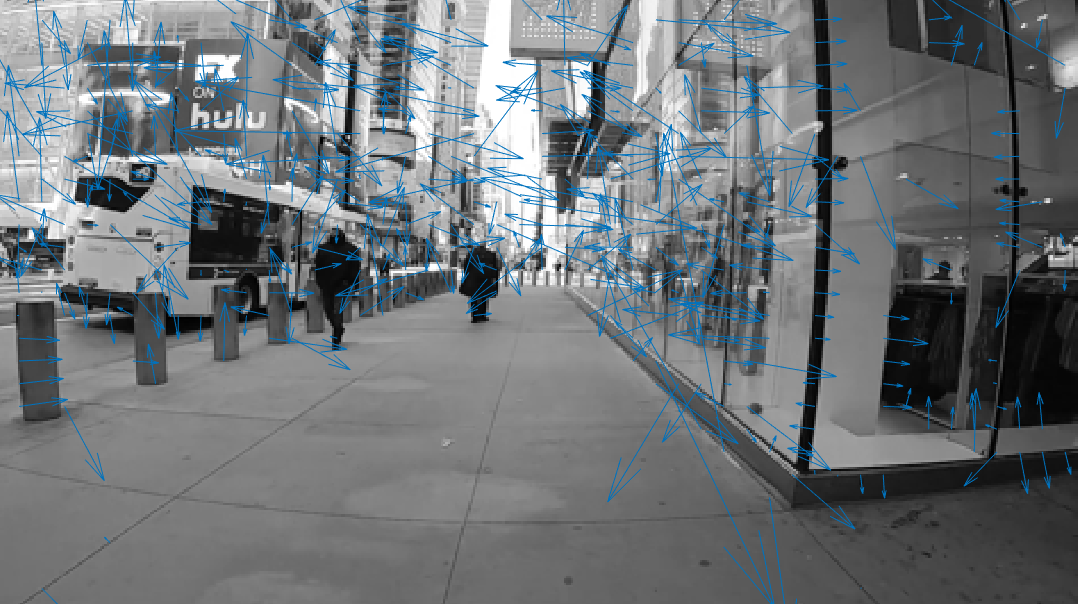
\includegraphics[width=0.4\linewidth]{./Figures/LK.png}}
\hspace{5mm} %
\subfloat[Horn-Schunck method]{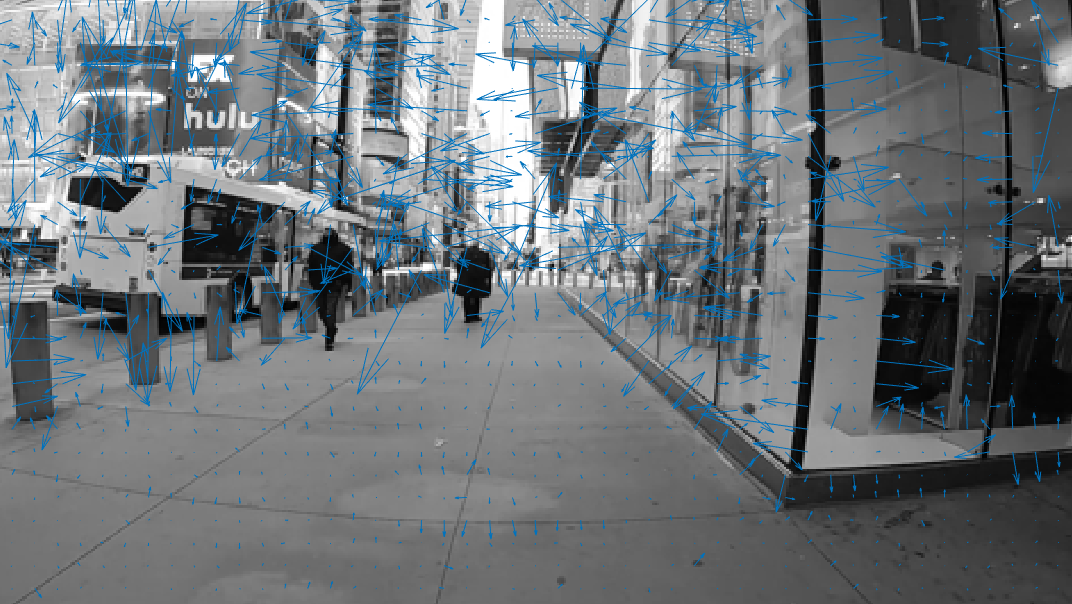
\includegraphics[width=0.4\linewidth]{./Figures/HS.png}}
\caption{Optical Flow estimates using MATLAB in-built function.}
\label{fig:flow}
\end{figure}

By horzontally stacking each of the flow velocities vectors along $x$-direction, matrix $F_X$ is constructed. Similarly by stacking flow velocities along $y$-direction, matrix $F_Y$ is constructed. Rows of the matrix represent variables, while columns represent measurements. These matrices are then singularly decomposed. The semilogy plot of energy contained in each of the singualr modes shows that these modes are compact and contain low-energy. This makes sense since there are large number of variables (each pixel essentially is a variable).

\begin{figure}[!b]
\centering
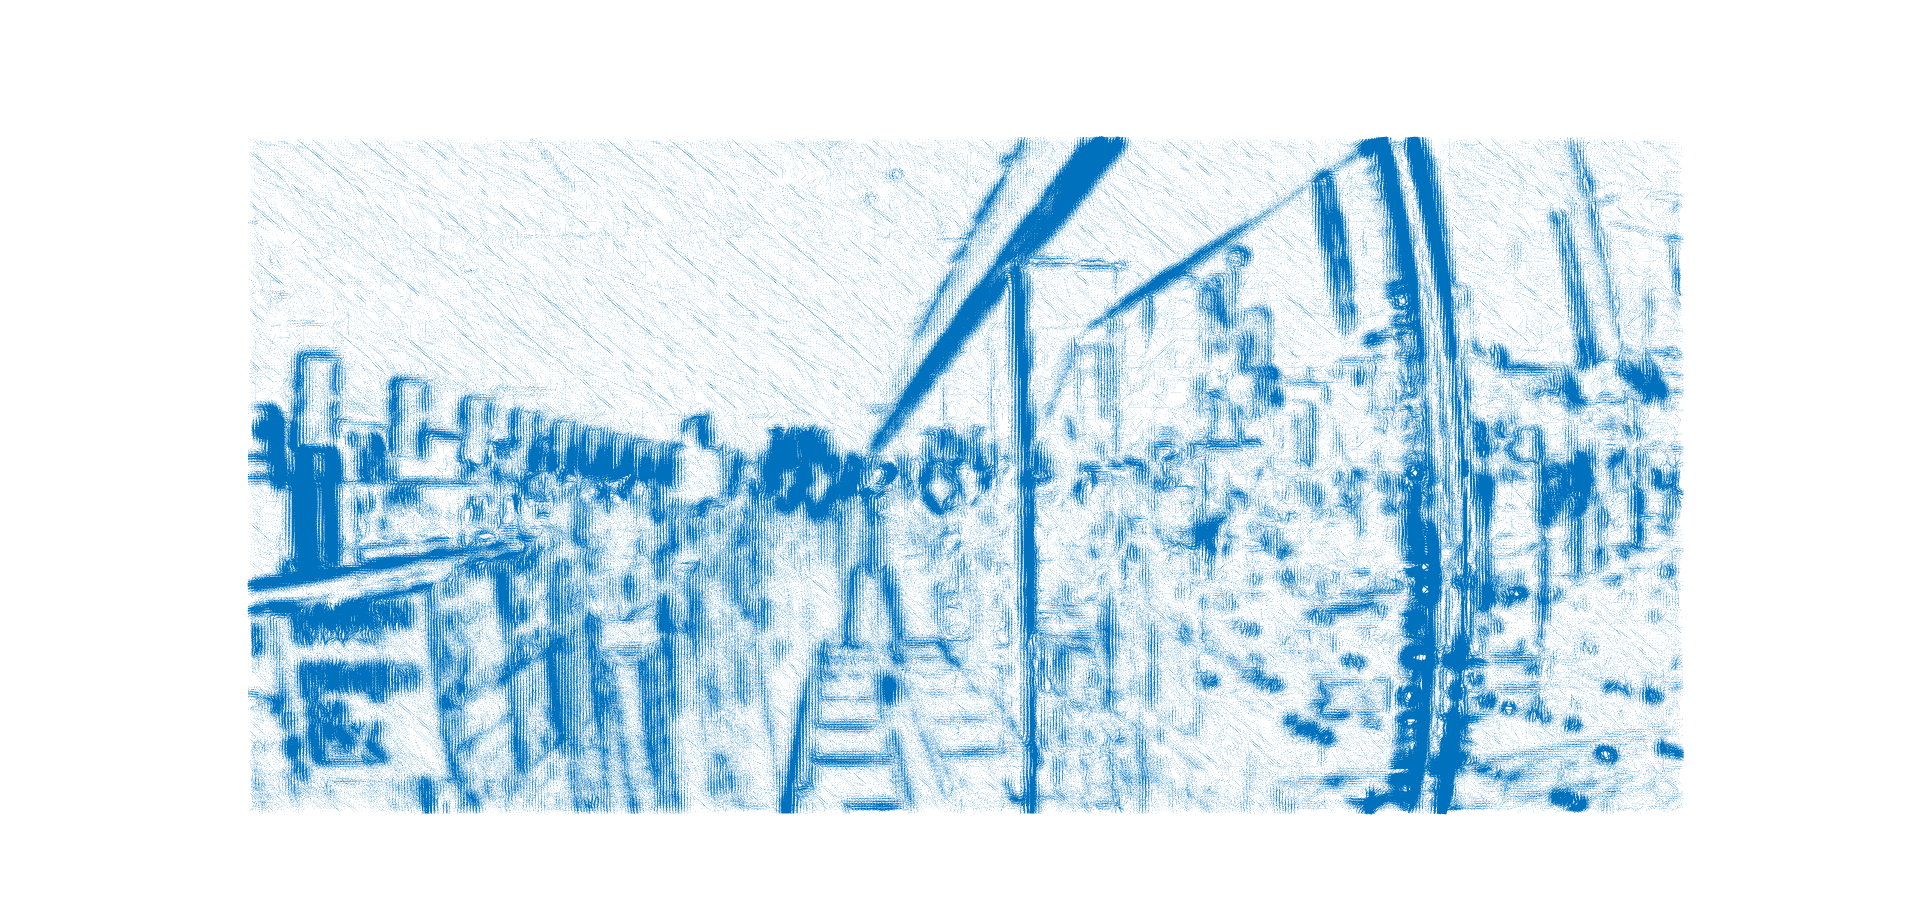
\includegraphics[width=\linewidth]{./Figures/velocity.png}
\caption{A vector field representing flow velocities at each pixel point between two consecutive frames.}
\label{fig:vel}
\end{figure}

\begin{figure}[!t]
\centering
\subfloat[$4^{\text{th}}$ dominant mode along $x$-direction.]{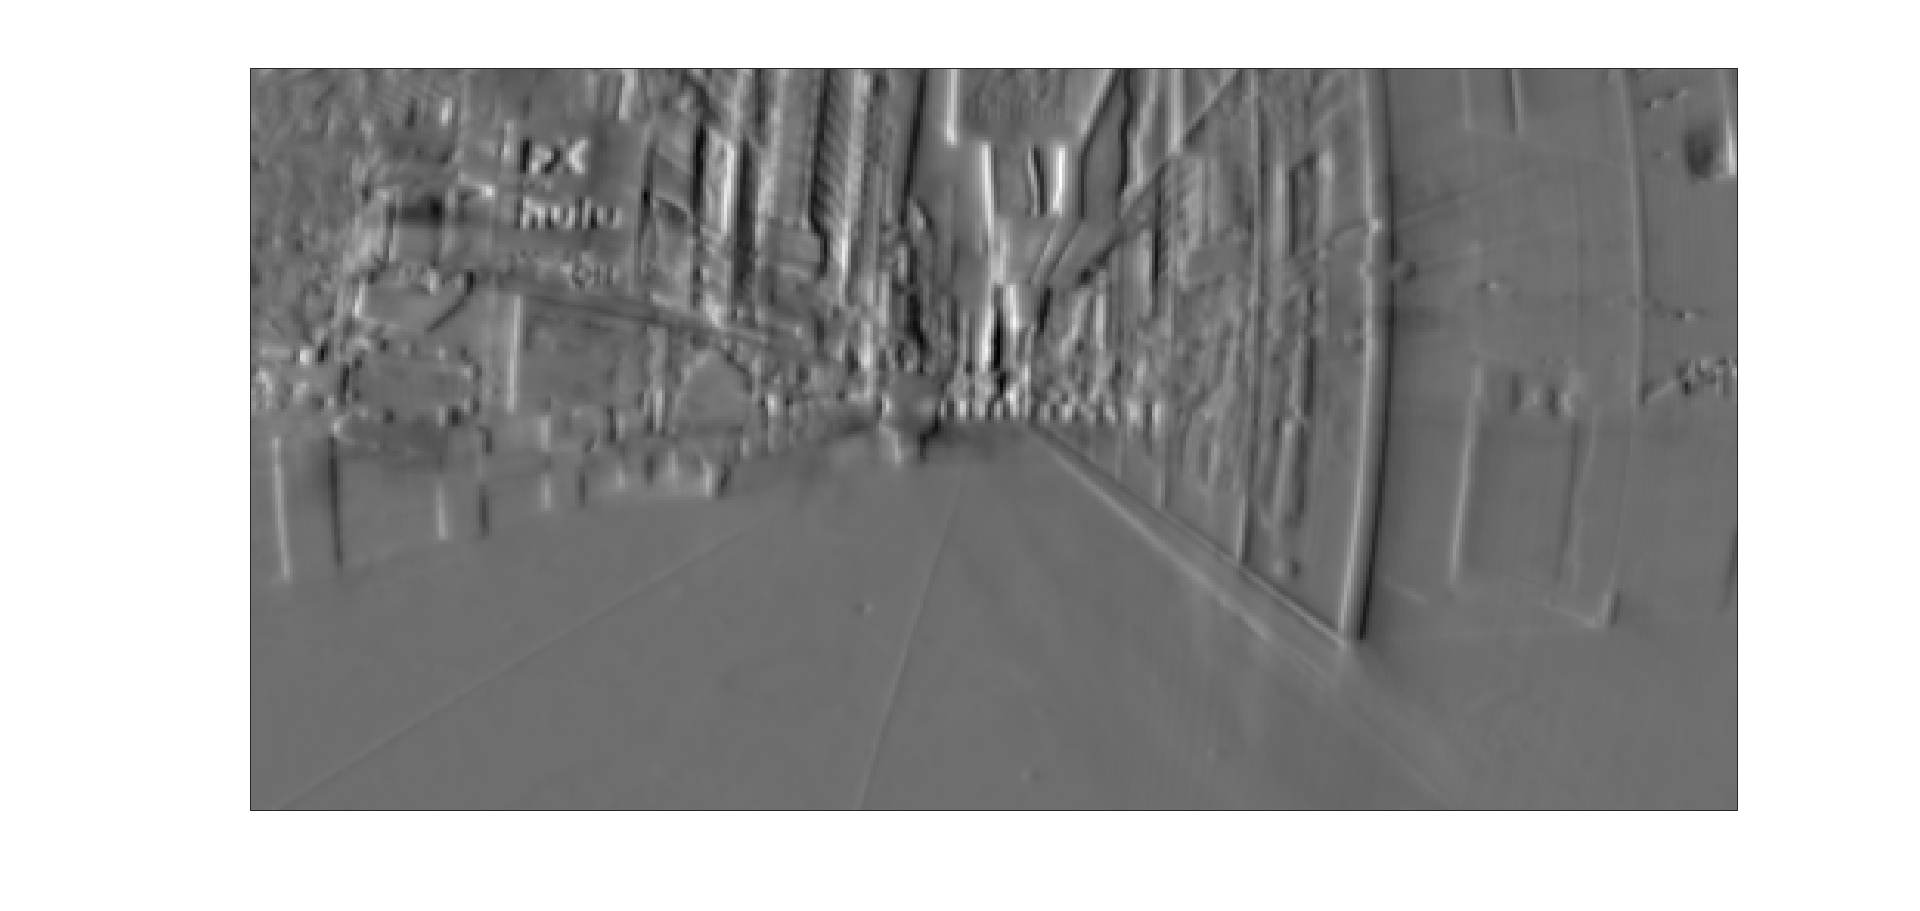
\includegraphics[width=0.5\linewidth]{./Figures/mode4_x.png}}
\subfloat[$2^{\text{nd}}$ dominant mode along $y$-direction.]{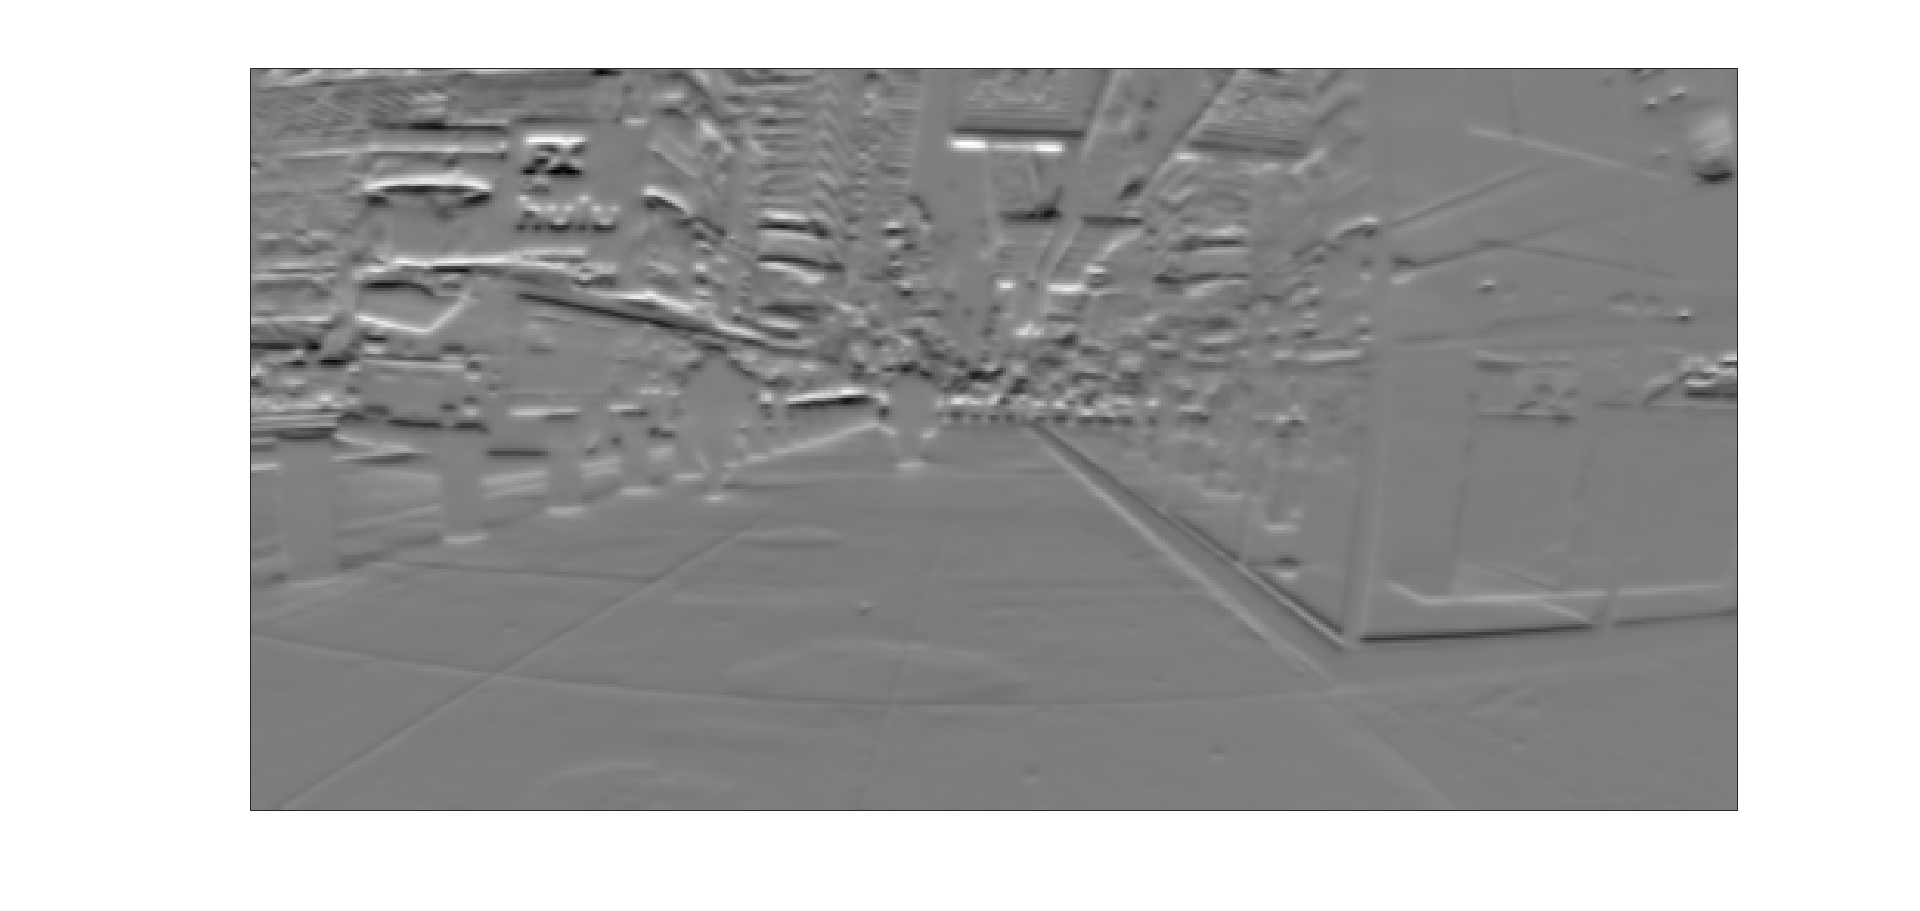
\includegraphics[width=0.5\linewidth]{./Figures/mode2_y.png}}
\caption{Dominant modes that capture horizontal and vertical motion of objects in the camera. (relative motion)}
\label{fig:mode}
\end{figure}

\begin{figure}[!t]
\centering
\subfloat[$1^{\text{st}}$ dominant mode along $x$-direction.]{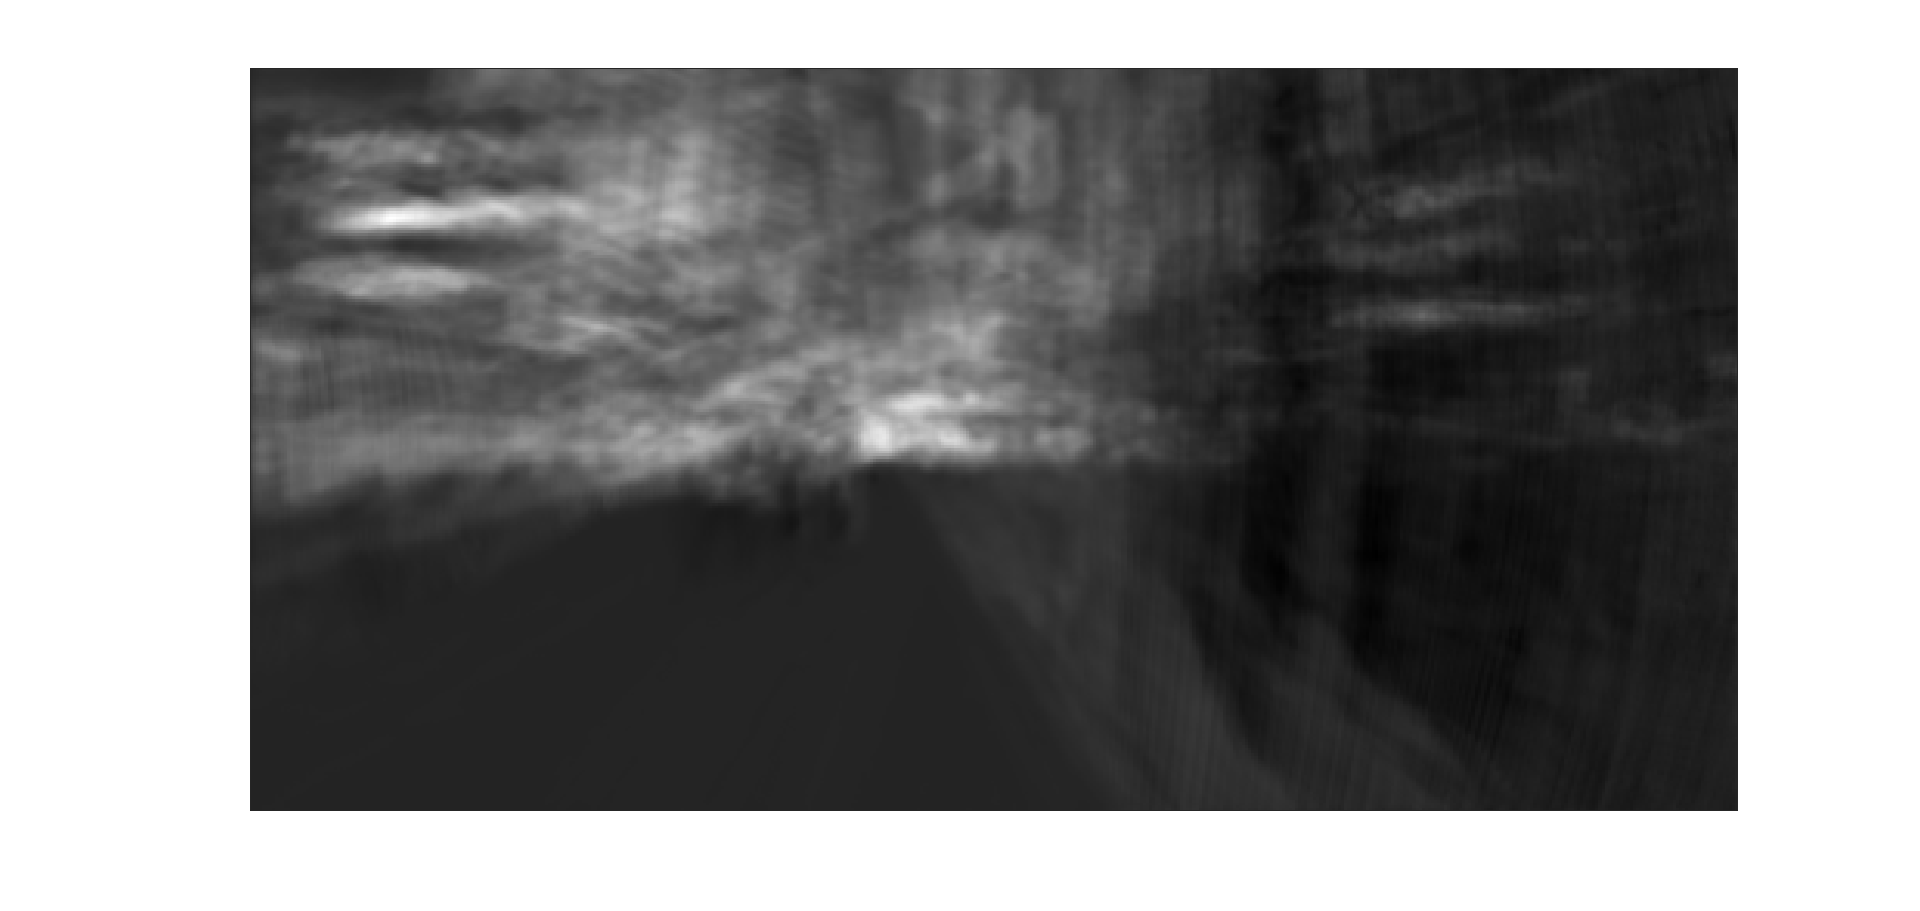
\includegraphics[width=0.5\linewidth]{./Figures/mode1_x.png}}
\subfloat[$1^{\text{st}}$ dominant mode along $y$-direction.]{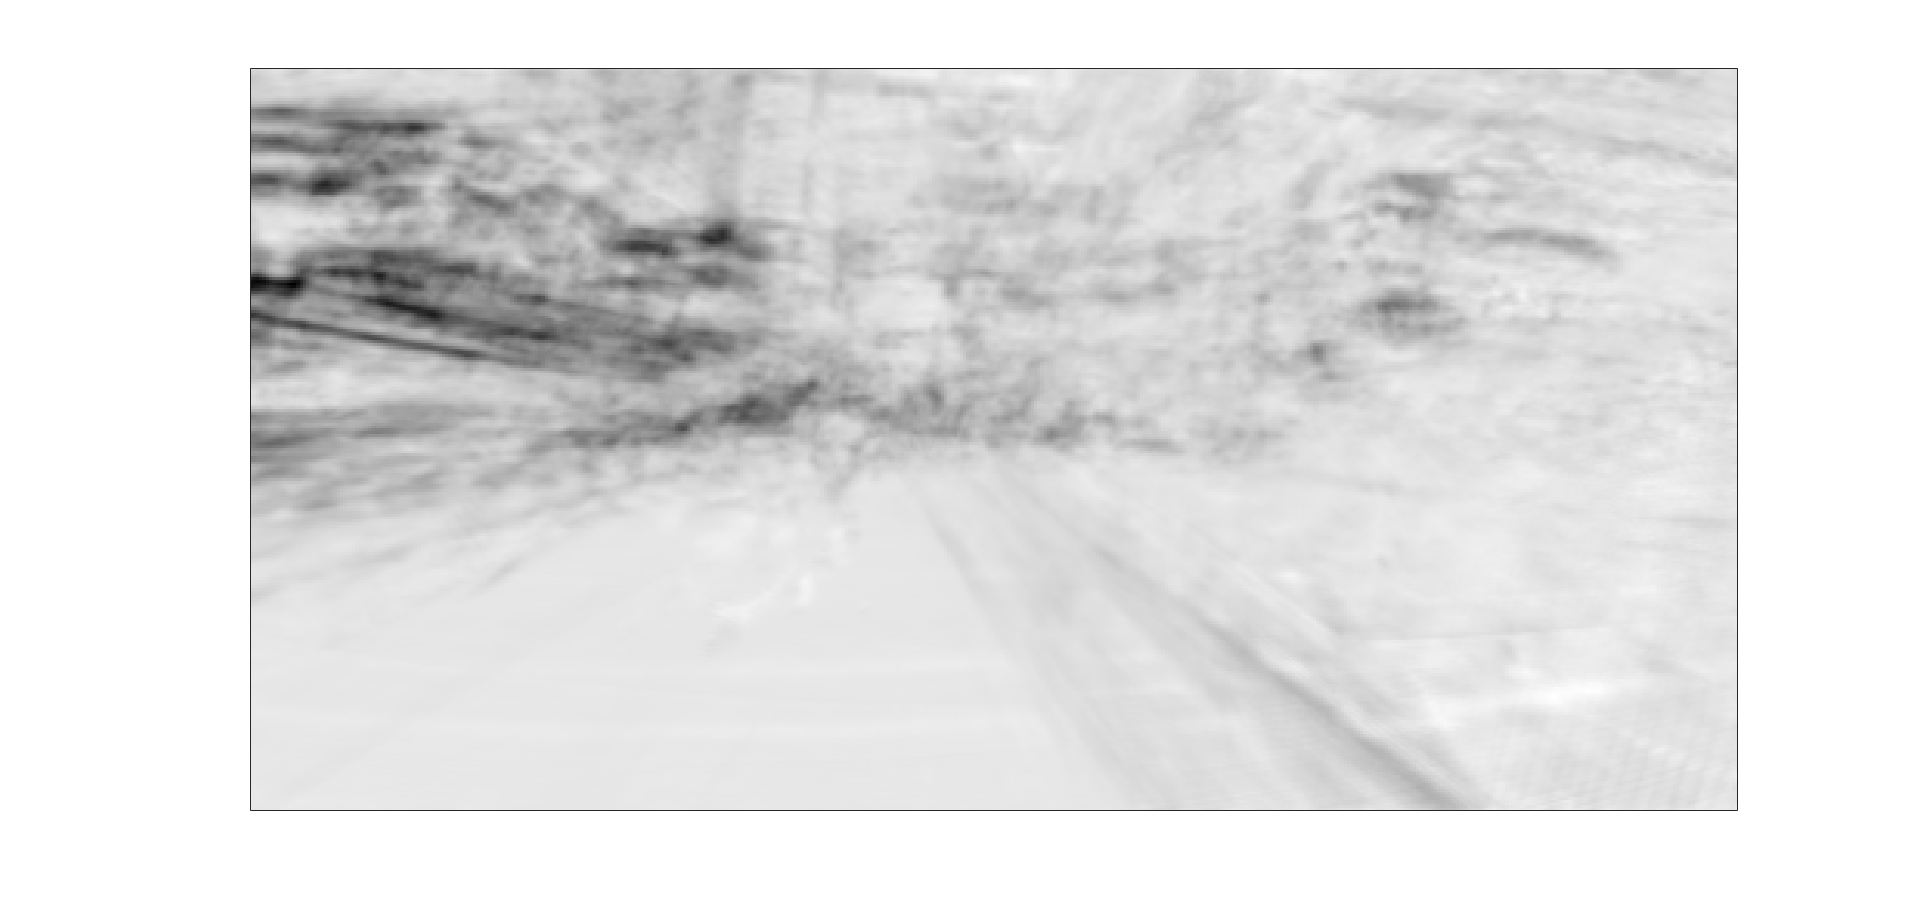
\includegraphics[width=0.5\linewidth]{./Figures/mode1_y.png}}
\caption{Most dominant modes in the SVD.}
\label{fig:mode2}
\end{figure}

Figure \ref{fig:mode} shows the dominant mode that captures the horizontal and vertical motion of pixels in the scene, due to the motion of the camera. They are exactly what we would have expected. A horizontal motion is best captured by tracking the movement of features on vertical lines/structures. Similarly, a vertical motion is best captures by tracking features on the horizontal lines. Thus, these two modes represent the forward motion of the person with camera. The other $299$ modes can represent numerous features like motion of the objects themselves in the video and noise. Figure \ref{fig:mode2} shows the most dominant modes in each direction. The black region in figure (a) indicates $0$ flow velocities. This coincides with the region in the image where buildings are and they do not move themselves. Thus this mode indicates the motion of objects itselfs like buses, cars and pedestrians. It is not clear what figure (b) is representing as the pattern is not obvious.

My initial intent was to similarly identify the mode associated with walking, but it seems there is no clear way to find that out. The problem itself is little ambigious because a pixel (object) can move up by either moving up itself, camera moving down or camera moving forward. The questions then is how do we distinguish those cases. On this paper, I was not able to figure that out.

The next stage was to reconstruct the video by using a low-rank approximation of the flow velocity matrix ($F_X(r)$,$(F_Y(r)$).

\begin{align*}
F_X(r) = U_{X}[:,1:r]S_X[1:r,1:r]U_X[:,1:r]' + \bar{X} \\
F_Y(r) = U_{Y}[:,1:r]S_Y[1:r,1:r]U_Y[:,1:r]' + \bar{Y}
\end{align*}
where $\bar{X}$ and $\bar{Y}$ are means of the flow velocities along $x$ and $y$ directions.

Each image was then warped using the MATLAB in-built 2D interpolation function \emph{interp2}. The following relation was used to find the warping matrix.
\begin{align*}
X_p = X - f_X \\
Y_p = Y - f_Y \\
\end{align*}
where $(X,Y)$ defines the mashgrid of pixel points in the image space and $(f_x,f_Y)$ are flow velocity matrices of a frame. The approximations were decent, as seen in previous homeworks. Figure \ref{fig:reconstructed} shows the original and reconstructed image with first $20$ principal modes of both SVD.


\begin{figure}[!t]
\centering
\hspace{2mm} %
\subfloat[Original Image]{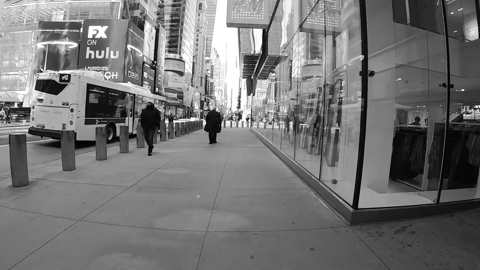
\includegraphics[width=0.4\linewidth]{./Figures/original.png}}
\hspace{15mm} %
\subfloat[Reconstructed Image.]{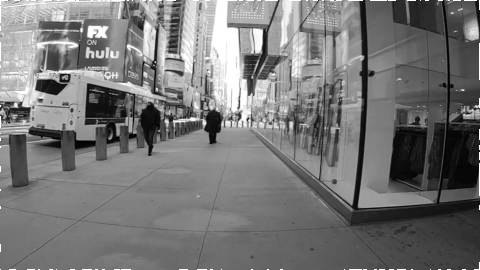
\includegraphics[width=0.4\linewidth]{./Figures/reconstructed.png}}
\caption{Image reconstruced with 20-rank approximation of flow velocity matrices.}
\label{fig:reconstructed}
\end{figure}


% Summary, Conclusions and Future Work
\section{Summary and Conclusions}
In this paper, Singular Value Decomposition was used to stabilize video captured with a hand held camera while the person is walking. The idea was to find the mode associated with walking and isolate that mode from the SVD. However, it became clear this was not as easy as it sounds. The paper discusses different principal modes that were captured and how we can study some of them and identify what they represent in the scene. Lucas-Kanade and Horn-Schunck methods of solving optical flow equations were introduced and implemented using MATLAB built-in functions. The video was reconstructed using a low-rank approximation of flow velocity matrices.

\pagebreak
% Appendices
\begin{appendices}

% MATLAB Functions
\section{MATLAB Functions}
Some important MATLAB functions used during the implementation.
\begin{itemize}
\item \texttt{[U,S,V] = svd(A)} performs a singular value decomposition of matrix A, such that A = U*S*V'.
\item \texttt{B = repmat(A,r1,...,rN)} specifies a list of scalars, r1,..,rN, that describes how copies of A are arranged in each dimension. When A has N dimensions, the size of B is size(A).*[r1...rN]. For example, repmat([1 2; 3 4],2,3) returns a 4-by-6 matrix.
\item \texttt{imagesc(C)} displays the data in array C as an image that uses the full range of colors in the colormap
\item \texttt{movegui(f,position)} moves the figure f to the specified screen location.
\item \texttt{p = uipanel} creates a panel in the current figure and returns the Panel object. If there is no figure available, MATLAB® calls the figure function to create one.
\item \texttt{opticFlow = opticalFlowLK} returns an optical flow object that you can use to estimate the direction and speed of the moving objects in a video. The optical flow is estimated using the Lucas-Kanade method.
\item \texttt{opticFlow = opticalFlowHS} returns an optical flow object that you can use to estimate the direction and speed of the moving objects in a video. The optical flow is estimated using the Horn-Schunck method.
\item \texttt{flow = estimateFlow(opticFlow,I)} estimates optical flow between two consecutive video frames.
\item \texttt{imwrite(A,filename)} writes image data A to the file specified by filename, inferring the file format from the extension. imwrite creates the new file in your current folder.
\item \texttt{v = VideoReader(filename)} creates object v to read video data from the file named filename.
\item \texttt{Vq = interp2(X,Y,V,Xq,Yq)} returns interpolated values of a function of two variables at specific query points using linear interpolation.
\item \texttt{h = quiver(...)} A quiver plot displays velocity vectors as arrows with components (u,v) at the points (x,y).
\end{itemize}

\pagebreak
% MATLAB Codes

\section{MATLAB Code}
\href{https://github.com/cssubedi/AMATH-582}{The code is published on the github repository AMATH-582 under Video Stabilization.} \\

\textbf{MATLAB code for Eigenfaces problem.}
\lstinputlisting[style=Matlab-editor]{video_stabilization.m}

\end{appendices}
\end{document}
